\documentclass{article}
\usepackage[utf8]{inputenc}
\usepackage{amsmath}
\title{Report Lab DC: Digital Systems}
\author{Henning Schei}
\date{March 2016}
\usepackage{natbib}
\usepackage{graphicx}
\usepackage{listings}
\usepackage{color}
\usepackage{float}
\definecolor{dkgreen}{rgb}{0,0.6,0}
\definecolor{gray}{rgb}{0.5,0.5,0.5}
\definecolor{mauve}{rgb}{0.58,0,0.82}

\lstset{frame=tb,
  language=VHDL,
  aboveskip=3mm,
  belowskip=3mm,
  showstringspaces=false,
  columns=flexible,
  basicstyle={\small\ttfamily},
  numbers=none,
  numberstyle=\tiny\color{gray},
  keywordstyle=\color{blue},
  commentstyle=\color{dkgreen},
  stringstyle=\color{mauve},
  breaklines=true,
  breakatwhitespace=true,
  tabsize=3
}
\begin{document}

\maketitle


\section{Refinement of a VHDL model for synthesis}

\begin {itemize}
\item The target clock period is 2.0 nm, so the clock freq is 1/2.0 = 5e+8 = 500 MHz.
\item The input and output delay is 0.5 ns
\item The synthesis gives the following errors \\
Error:  ../g1.vhd:27: WAIT statement inside FOR loop is not supported. (ELAB-996)\\
Error:  ../g1.vhd:27: WAIT statement inside FOR loop is not supported. (ELAB-996)\\

There are wait statements on several occations in the process. These lines needs to be rewritten to be synthesizable. Although not only the wait-statement is the only thing preventing this process to be synthesizeable: The inner for-loop has a variable length and that is not synthesizeable. I did the following.


\begin{lstlisting}

  p: process(clk,rst)
  begin
    if rst = '1' and clk = '1'  then
      s   <= '0';
      cnt <=  0;
    elsif clk = '1' and clk'event then
      if a = '1' and (cnt = 0 or cnt = 31) then
        cnt <= 1;
      elsif cnt = 31 then
        cnt <= 0;
      elsif cnt /= 0 then
        cnt <= cnt +1;
      end if;

    case cnt is
        when 1 to 16 => s <= '1';
        when 25 to 28 => s <= '1';
        when 31 => s <= '1';
        when others => s <= '0';
      end case;
    end if ;
  end process p;
\end{lstlisting}

\item 
\begin{figure}[H]
\begin {center}
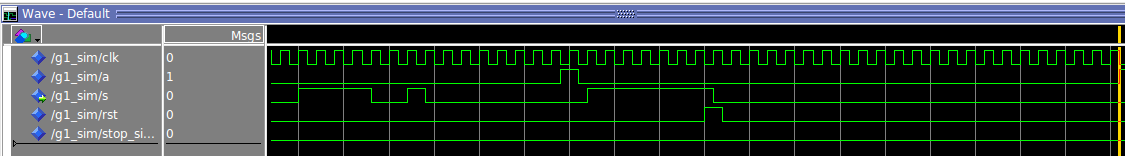
\includegraphics[scale=0.4]{syncrst.png}
\caption{wave diagram showing sync reset}
\end{center}
\end{figure}








\end {itemize}



\section {Synthesis reports}
\begin{itemize}
\item The silicon area of the synthesized circuit is 102 $\mu m^2$.
\item According to the model, it should be 5 DFFs. And it's the same as in the html page. The cnt-varivale are counting from 0 to 31, such that we need at least log2(32) = 5 dff's. 

 
\item \begin{tabular}{ | l | p{5cm} |}
    \hline
    The critical path.\\ \hline U66/Y (XOR2X1RVT)\\ \hline U65/Y (XOR2X1RVT)\\ \hline U63/Y (AO22X1RVT) \\ \hline U51/Y (INVX0RVT) \\ \hline U49/Y (XNOR2X1RVT) \\ \hline U47/Y (NAND2XRVT) \\ \hline U46/Y (XOR2X1RVT) \\ \hline U39/Y (AO22X1RVT) \\ \hline \end{tabular}

\item  The endpoint is the cnt\textunderscore reg[0]/D (DFFARX1\textunderscore RVT)       
\item  According to the synthezis report, the 1.04 ms long. 
\item  The correspongding maximum clock frequency is 961.5


\end{itemize}


\section {GUI}
\begin{figure}[H]
 \begin {center}
  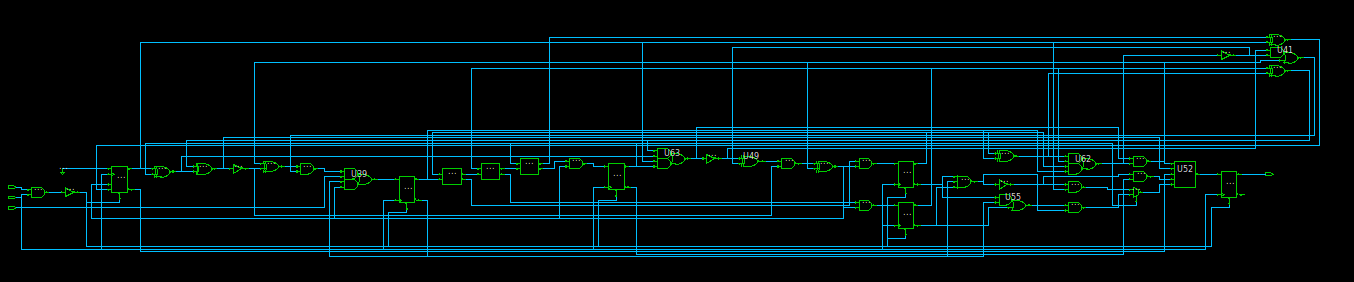
\includegraphics[scale=0.3]{sirquit.png}
  \caption{Circuit}
  \end{center}
\end{figure}


\section {Improving the design}




%Startpoint: cnt_reg[0] (rising edge-triggered flip-flop clocked by clk)
%  Endpoint: cnt_reg[0] (rising edge-triggered flip-flop clocked by clk)
%  Path Group: clk
%  Path Type: max
%
%  Des/Clust/Port     Wire Load Model       Library
%  ------------------------------------------------
%  g1                 ForQA                 saed32rvt_tt0p85v25c
%
%  Point                                    Incr       Path
%  -----------------------------------------------------------
%  clock clk (rise edge)                    0.00       0.00
%  clock network delay (ideal)              0.00       0.00
%  cnt_reg[0]/CLK (DFFARX1_RVT)             0.00       0.00 r
%  cnt_reg[0]/Q (DFFARX1_RVT)               0.17       0.17 r
%  U66/Y (XOR2X1_RVT)                       0.15       0.32 f
%  U65/Y (XOR2X1_RVT)                       0.15       0.47 r
%  U63/Y (AO22X1_RVT)                       0.08       0.55 r
%  U51/Y (INVX0_RVT)                        0.05       0.60 f
%  U49/Y (XNOR2X1_RVT)                      0.11       0.72 f
%  U47/Y (NAND2X0_RVT)                      0.06       0.78 r
%  U46/Y (XOR2X1_RVT)                       0.15       0.93 f
%  U39/Y (AO22X1_RVT)                       0.10       1.03 f
%  cnt_reg[0]/D (DFFARX1_RVT)               0.01       1.04 f
%  data arrival time                                   1.04
%
%  clock clk (rise edge)                    2.00       2.00
%  clock network delay (ideal)              0.00       2.00
%  cnt_reg[0]/CLK (DFFARX1_RVT)             0.00       2.00 r
%  library setup time                      -0.05       1.95
%  data required time                                  1.95
%  -----------------------------------------------------------
%  data required time                                  1.95
%  data arrival time                                  -1.04
%  -----------------------------------------------------------
%  slack (MET)                                         0.90

\end{document}

